%*********************第三章******************
\chapter{跟踪器中``目标候选''的作用分析和优化}
\label{chapijcv}

\section{引言}
在``目标候选''(原英语术语为``Detection Proposal'',这里采用意译)方法出现之前,
物体检测领域通常使用``滑动窗口(Sliding Window)''的方式来检测物体\upcite{slidingdetect1, slidingdetect2}。
滑动窗口指的是无视输入图像的实际内容,直接用一个窗口扫描整幅图像(在输入图像中不断滑动),
同时不断利用分类器判断窗口中的图像块是否包含目标物体。
由于物体可能是任意大小的,上述过程需要使用不同尺度和宽高比的窗口重复多次。
据统计,在常用的物体检测数据集\upcite{voc2007, coco}上,
一次单尺度的滑动窗口就会产生$10^4\sim 10^5$个候选窗口。
若引入不同的尺度和宽高比,窗口数目将高达$10^6\sim 10^7$\upcite{dpsurvey, dpsurvey2}。
因为整个物体检测过程所需时间等于一个窗口的分类时间乘以窗口数目,
巨大的候选窗口数量严重地限制了用于检测的分类器的复杂度,
使得物体分类领域的先进方法难以应用于物体检测任务。

为了减少滑动窗口所带来的巨大计算压力,``目标候选''方法应运而生。
所有目标候选方法均基于同一个假设,即任何包含物体的图像区域都具有一种共同的视觉特性,
该特性使得这些区域能够和背景区域区别开来。
因此,一定存在某种方法,能够以一幅图像为输入,然后输出一系列很可能包含着物体的候选区域。
这样的方法即是目标候选方法。
如果目标候选方法的输出能够足够准确地覆盖绝大部分物体,
且输出的候选区域数目远小于滑动窗口产生的(这在物体检测领域被称作``高召回率''),
那么物体检测过程将获得巨大的速度提升。
此外,使用更加复杂而准确的分类器也成为了可能,从而检测精度也将大幅提高。
经过多年的发展,目标候选方法已经具备了上述作用,在物体检测领域占有重要地位。
无论在经典的PASCAL数据集\upcite{voc2007}上,还是在庞大的ImageNet数据集\upcite{imagenet}上,
当前排名靠前的物体检测器均使用了目标候选方法\upcite{rcnn, detector1, detector2, detector3}。
实际的应用证明,除了上述作用以外,目标候选方法还能减少``错误肯定(False Positive)''对分类器的干扰,
从而进一步提升物体检测的准确性。

上一章中,通过将目标候选生成器EdgeBoxes不加修改地嵌入KCF跟踪器中,
获得了引人注目的尺度和宽高比适应力提升。
其中的整体方法是通用的,可用于将任何跟踪器和任何目标候选生成器进行结合。
该方法的本质在于,将目标候选生成器作为跟踪器运动模型的补充。
在理想情况下,即所有物体都被目标候选准确覆盖时,这种补充作用将会非常有效:
对于密集的运动模型,目标候选的灵活性将弥补运动模型固化的采样模式;
而对于随机的运动模型,目标候选对物体的感知力将弥补随机采样可能错过跟踪目标这一最大缺陷。
但是,上述的理想情况是难以满足的,目标候选生成器必然存在误差甚至错误,
而目前还尚未有任何文献讨论过目标候选的质量对于跟踪精度的影响。
此外,上一章仅对EdgeBoxes进行了参数调优,并没有对本质算法进行面向跟踪任务的优化,
因此KCFDP的性能还有着一定的提升空间。
本章将针对上述两个问题进行深入的研究。
一方面,通过将多个目标候选生成器逐一地与上一章的跟踪器进行结合,揭示了目标候选的质量和跟踪精度间有着密切的关系。
另一方面,通过为EdgeBoxes加入``背景抑制''这一优化步骤,以极低的时间开销提升了EdgeBoxes对于跟踪任务的适应性,
从而提高了整体跟踪性能。

本章的内容安排如下:
第2节介绍与本章相关的研究工作,主要是典型的目标候选生成器及它们在视觉跟踪中的应用;
第3节介绍目标候选生成器EdgeBoxes,并对其进行面向跟踪任务的优化;
第4节介绍如何将其它5个目标候选生成器和跟踪器相结合;
第5节进行实验,将分析目标候选质量对于跟踪精度的影响,并评测优化后的EdgeBoxes带来的性能提升;
第6节进行本章小结。



\section{相关研究}
``兴趣点检测(Interest Point Detection)\upcite{interestpoint1, interestpoint2}''和
``显著性检测(Saliency Detection)\upcite{saliency1, saliency2}''
在目标候选方法出现之前就是视觉领域重要的研究课题。
它们和目标候选方法有着相似的动机,但研究背景有所不同。
兴趣点检测和显著性检测主要依据仿生学原理,研究人的视觉系统规律,目的是从图像中找出能够吸引人类注意的突出区域和特别区域。
因此,它们常被用于物体分类、图像检索、图像对比等领域,以大幅减少计算开销。
而目标候选方法专注于物体检测,其本质在于研究物体所在的图像区域(而不是视觉上的显著区域)所具有的视觉特性,
即``物体性(Objectness)''。

目标候选方法在近几年发展迅速,形成了两种主要类型,
即``区域分组(Grouping)''类方法和``窗口评分(Window Scoring)''类方法\upcite{dpsurvey}。

SelectiveSearch\upcite{selectivesearch}是一种典型的区域分组方法,它首先利用边缘提取将图像划分为大量``超像素(Super Pixel)'',
然后使用贪心法将超像素进行合并,得到可能包含物体的各个区域。超像素合并的标准基于人工设计的特征和相似性度量,无需任何训练过程。
SelectiveSearch的应用在当前是最为广泛的,R-CNN\upcite{rcnn}和Fast R-CNN\upcite{fastrcnn}均基于它进行物体检测。
CPMC\upcite{cpmc}首先通过设置不同的``种子点(Seed)''和分割参数来进行多次图像分割(Graph Cut),
然后根据多种中层图像特征,将分割得到的图像分块进行筛选和排序,以得出可能包含物体的区域。
Geodesic\upcite{geodesic}会预先训练一个用于在图像中放置种子点的分类器。
基于该分类器放置的种子点,Geodesic将进行前背景分割,并利用分割结果计算``带符号的测地线距离变换(Signed Geodesic Distance Transformation,SGDT)''。
最后,超像素将根据不同的SGDT等级设置进行合并,得到目标候选区域。

与区域分组类的方法不同,窗口评分类方法通常产生密集的候选窗口,然后对候选窗口进行评分,以计算窗口内包含物体的可能性。
一些窗口评分方法甚至仍采用滑动窗口的方式来产生候选窗口,但是由于此时无需进行实际的物体分类,
其评分函数可以设计得非常高效,足以满足时效性要求。
Objectness\upcite{objectness}通常被认为是最早的目标候选生成器。
它首先进行显著性检测,并在显著区域附近提取大量候选窗口,
然后基于多种线索,利用贝叶斯框架对这些窗口的``物体性''进行评分。
Objectness的评分函数所采用的线索包括颜色、边界、位置、大小、以及非常有效的``超像素跨越''线索。
Bing\upcite{bing}的核心部分是一个以``规范化梯度(Norm of Gradients)''为输入特征的线性分类器。
经过在大型物体检测数据集上的训练,该分类器能够判断图像块内包含物体的概率。
通过对规范化梯度这一特征进行二进制近似,该线性分类器可变得极其高效,仅需几个原子操作即可完成。
因此即使Bing采用滑动窗口的方式提取候选窗口,其效率仍然是目前最高的。

上一章和本章所使用的EdgeBoxes\upcite{edgeboxes}也属于窗口评分类方法。
它首先进行边缘(Edge)提取,然后将边缘组合成边缘组(Edge Group),再考虑边缘组组成的物体边界(Contour)。
EdgeBoxes也采用了滑动窗口的方式,并且在给候选窗口评分时,认为完全包含在窗口内的边界数量就是``物体性''的体现。
上一章已经展示了EdgeBoxes在跟踪器中的巨大作用,
但同时也暴露出它的一些缺陷。
与物体检测任务不同,视觉物体跟踪仅关注被跟踪的目标物体,且对目标候选的准确度要求更高。
但是在跟踪场景下,EdgeBoxes很容易被非目标的物体边界,如属于背景、遮挡物、其它物体等的边界,所干扰,
从而生成不够准确甚至错误的目标候选。

就本文所知,最早将目标候选方法应用于物体跟踪的是上一章对应的论文\upcite{kcfdp}。
之后,目标候选在视觉跟踪过程中的作用得到了广泛的研究和开发\citep{proposalSelect, adobing, ebt, rpnt, moca}。
不同于上一章的KCFDP\upcite{kcfdp},ADOBING\upcite{adobing}和\cite{proposalSelect}中的方法均没有
将目标候选作为运动模型的补充,而是将目标候选生成器所获取的``物体性''作为额外的跟踪依据,用于增强跟踪器的观察模型。
ADOBING\upcite{adobing}在初始化跟踪器时,
会利用自适应SVM\upcite{adaptivesvm},对Bing的分类器进行面向被跟踪目标的修正。
修正后的Bing将作为观察模型的一部分,用于识别跟踪目标。
类似于ADOBING,\cite{proposalSelect}将EdgeBoxes的评分策略加入了跟踪器的辨别模型中,以更准确地区分目标物体和背景。
为了解决视觉跟踪中偶发的偏移问题,MOCA\upcite{moca}会周期性地根据``视觉显著性图''提取候选区域并进行辨别。
而在``视觉显著性图''中提取候选区域的过程也可以看作是一种目标候选生成器,
并且它在MOCA中的作用也是弥补原运动模型的不足。
EBT\upcite{ebt}和RPNT\upcite{rpnt}更进一步,它们直接使用修改后的目标候选生成器作为运动模型。
EBT在EdgeBoxes之上加入了一个针对跟踪目标的线性SVM分类器,以将目标候选重新排序,
使得生成的目标候选不仅包含``物体性'',还具有与跟踪目标的相似性。
RPNT使用在物体检测数据集上训练得到的区域候选网络(Region Proposal Network,RPN)\upcite{rpn}作为运动模型,
同时也在前一帧目标位置周围进行随机采样。


\section{跟踪器中目标候选生成器的优化}
通过加入上一章\ref{featureintegrasec}节中的特征整合和鲁邦更新优化,
KCFDP的跟踪器部分获得了显著的精度和鲁棒性提升。
但是作为尺度和宽高比适应力的来源,目标候选生成器在跟踪过程中仍然具有决定性的作用。
例如,如果生成的目标候选质量普遍较差,那么即使具有最高相关滤波响应值的目标候选,也无法用于描述目标物体的位置和大小。
此外,过多错误或者偏差的目标候选还会增加相关滤波器的误判概率,尤其是在背景较为杂乱时。
更严重的是,当错误的目标候选被相关滤波器误判时,该目标候选将被用于更新跟踪器的模型,造成模型的污染,
从而可能导致跟踪偏离目标。
因此,对目标候选生成器进行优化也是十分必要的。

目标候选生成器通常是``类别无关''的,即是说,它们的设计初衷就是生成能够覆盖图像中所有物体的目标候选,
包括那些背景物体和``不起眼''(低显著性)的物体。
但是,当目标候选生成器被用于物体跟踪时,我们期望生成的目标候选能够尽量集中于目标物体。
由于EdgeBoxes将物体边界作为唯一的``物体性''判断依据,它生成的目标候选很可能包含非目标物体边界,例如来自背景物体、
遮挡物体和其它背景纹理的边界。
这样的目标候选是不准确的,将会包括非目标的物体或者偏离目标中心。
为了缓解EdgeBoxes的这一缺陷,本节将对其进行优化。
具体地,本节将在滑动窗口和对窗口评分之前,添加一个额外的``背景抑制''步骤,
使得最终生成的目标候选不仅更加集中于目标物体,还能更准确地包围目标物体。

\subsection{目标候选生成器EdgeBoxes}
EdgeBoxes的思想可以概括为:边缘像素很可能属于物体的边界,而包围着完整物体边界的矩形框则很可能包含物体。
之所以强调包围``完整物体边界'',是因为如果一条物体边界跨越了边界框,那么该边界所属的物体将不处于该边界框内。
基于上述思想,EdgeBoxes将根据``被完全包围在边界框内的物体边界数量''来对候选窗口进行评分。

对于一幅输入图像,EdgeBoxes首先使用结构化边缘提取器\upcite{structurededge}为每一个像素计算出边缘响应值和边缘方向。
然后在垂直于各像素边缘方向的方向上进行非极大值抑制(Non-Maximal Suppression,NMS),
仅保留该方向上具有最大边缘响应的像素。
随后将响应值低于$0.1$的像素滤除,并把剩下的像素称作``边缘像素''。
这些边缘像素的响应值记为$m_p$,方向记为$\theta_p$。

边缘像素(Edge)将被组合成边缘组(Edge Group)。
组合的方法为:从各个像素出发进行贪心搜索,不断地将8个方向上邻接的、且边缘方向差别最小的边缘像素加入到边缘组中。
每一次加入新的边缘像素,都将其边缘方向差别累加,直到积累到大于某阈值(这里设置为$\pi/2$)就停止组合过程。
最后,过短的边缘组还将被融入邻近的较长边缘组中。

从直观角度来讲,如果两个边缘组邻接,且趋向相同,那么它们很可能属于同一条物体边界(Contour);
反之,如果两者互相间隔,或者相邻但连接后形成大曲率曲线,那么它们很可能分属两条不同物体边界。
EdgeBoxes将两个边缘组属于同一条物体边界的可能性用``亲和度(Affinity)''来度量,其计算公式如下:
\begin{equation}
a(\textbf{s}_i,\textbf{s}_j)=|\cos(\theta_i-\theta_{ij})\cos(\theta_j-\theta_{ij})|^\gamma, \label{edge_affinity}
\end{equation}
其中$a(\textbf{s}_i,\textbf{s}_j)$代表边缘组$\textbf{s}_i$和$\textbf{s}_j$间的亲和度,
$\theta_{i}$和$\theta_{j}$分别是两个边缘组的平均边缘方向。
记两个边缘组的平均位置坐标为$x_i$和$x_j$,则上式中的$\theta_{ij}$就是从$x_i$到$x_j$所形成的直线方向。
显然,如果两个边缘组的平均方向($\theta_{i}$和$\theta_{j}$)与它们相连后的趋向($\theta_{ij}$)相近,
那么它们间将具有较大亲和度。
上式的$\gamma$用于调整亲和度对于方向的敏感度,这里设置为$2$。
此外,如果两个边缘组间隔$2$个像素以上,则亲和度设置为$0$。
EdgeBoxes将计算出任意两对边缘组间的亲和度,以用于窗口评分。
由于大部分的边缘组是互相间隔的,亲和度计算的实际开销并不大。

完成上述的边缘组提取和亲和度计算后,将进入滑动窗口和对各个窗口评分的过程。
在进行滑动窗口之前,为了提高计算效率,
EdgeBoxes会预先为图像中的每一个边缘组$\textbf{s}_i$计算出组内像素的总响应值,记为$m_i$。
然后为每个边缘组随机提取一个像素$\overline{x}_i$,并记录下来,以快速判断各边缘组是否在某窗口内。
滑动窗口的过程和控制参数已经在\ref{param_setup}节中介绍过了,这里不再赘述,仅详细介绍对一个窗口$b$的评分过程。
为了能够度量``被完全包围在边界框内的物体边界数量'',EdgeBoxes将为每个边缘组$\textbf{s}_i$计算一个权值$w_b(\textbf{s}_i)\in [0,1]$。
它代表着$\textbf{s}_i$所在的物体边界被完全包含在窗口内的概率。
对于所有跨过窗口$b$的边界的边缘组,记它们组成的集合为$S_b$。
显然如果$\textbf{s}_i\in S_b$,则应有$w_b(\textbf{s}_i)=0$。
类似的,对于任何$\textbf{s}_i$,如果对应的$\overline{x}_i\notin b$,则$w_b(\textbf{s}_i)=0$,因为此时$\textbf{s}_i$只有两种可能:
全部处于窗口$b$之外,或者$\textbf{s}_i\in S_b$。
对于余下的边缘组,即$\overline{x}_i\in b$且$\textbf{s}_i\notin S_b$,按下式计算其$w_b(\textbf{s}_i)$:
\begin{equation}
w_b(\textbf{s}_i)=1-\max_\textbf{T}{\prod_{j=1}^{|\textbf{T}|-1}a(\textbf{t}_j,\textbf{t}_{j+1})}. \label{wbsi}
\end{equation}
上式中,$\textbf{T}$代表一系列边缘组(或者称为一条``路径''),它从某一边缘组$\textbf{t}_1\in S_b$出发,
至$\textbf{t}_{|\textbf{T}|}=\textbf{s}_i$结束,长度为$|\textbf{T}|$。
如果不存在这样的路径,则$w_b(\textbf{s}_i)=1$。
也即是说,上式将找出一条从$\textbf{s}_i$到窗口$b$边界的具有最大亲和度的路径,
然后根据这条路径是一条物体边界的概率(即路径上边缘组亲和度的乘积),对$w_b(\textbf{s}_i)$进行惩罚。
由于大部分边缘组间的亲和度为$0$,因此上述过程也较为高效。

获得$w_b$后,即可为窗口$b$进行评分,评分函数为:
\begin{equation}
	h_b = \frac{\sum_{i}w_b(\textbf{s}_i)m_i}{2(b_w+b_h)^\kappa} - \frac{\sum_{p\in b^{in}}m_p}{2(b_w+b_h)^\kappa}. \label{edgeboxes-full}
\end{equation}
上式和上一节的公式\ref{edgeboxes}虽然形式上不同,但实质是相同的。
这里$i$不再代表像素,而是边缘组的编号。$m_i$为边缘组内像素的总响应值,而$m_p$为像素$p$的边缘响应值。
由于边缘并没有宽度,所以用于惩罚较大窗口的分母是基于周长而不是面积的。
目标候选生成器Objectness\upcite{objectness}已经证明,窗口中心部分的边界信息对于``物体性''几乎没有贡献,
因此评分函数最终将减去位于$b^{in}$内的全部像素的边缘响应值。

\subsection{使用背景抑制优化EdgeBoxes}
\label{backsuppresssec}
在KCFDP中,如图\ref{process}(b)所示,输入EdgeBoxes的图像块(尺度和宽高比检测窗口)
的中心位于KCF得出的``初步目标位置'',其尺度大于上一帧的目标大小。
鉴于优化后的KCF具有足够的准确性,并且目标物体的尺度变化通常慢于位置变化,
此时可以做出一个合理的假设:当前帧中的目标物体被完全包含在EdgeBoxes的输入图像块中。
显然,在这种情况下,若一条物体边界跨越了输入图像块的边界,那么该物体边界必然不属于目标物体。
这样一来,本节得到了一种可靠地判断非目标物体边界的方法。

如本节开头所述,跟踪任务中EdgeBoxes极易被非目标物体边界所干扰。
如果能够将非目标物体边界消除,那么EdgeBoxes生成的目标候选将集中于目标物体,且更加准确。
但是,上述对非目标物体边界的判断方法并不完美(物体大小发生剧烈变化时可能超出图像块的范围),
并且EdgeBoxes对边缘组是否属于同一边界的判断标准也存在误差(目标物体边缘组和非目标物体边缘组间也可能有较高亲和度),
因此本节仅对判断出的非目标物体边界进行``抑制'',称为``背景抑制(Background Suppression)'',
而不是彻底地去除非目标物体边界。

对于EdgeBoxes的输入图像块$\mathbf{z}$,在边缘组提取和亲和度计算之后,在滑动窗口和窗口评分之前,
本节将根据$\mathbf{z}$中各个边缘组属于非目标物体边界的可能性,对它们的边缘响应值进行惩罚,以达到背景抑制的目的。
对于$\mathbf{z}$内的每个边缘组$\textbf{s}$,首先计算它的``抑制因子(Suppression Factor)'':
\begin{equation}
\mu_\mathbf{z}(\textbf{s})=\frac{1}{4}\max_{\textbf{T}'}{\prod_{j=1}^{|\textbf{T}'|-1}a(\textbf{t}'_j,\textbf{t}'_{j+1})}. \label{sup_factor}
\end{equation}
该式和公式\ref{wbsi}十分相似,不同的是,$\textbf{T}'$代表的是从$\textbf{s}$出发到达输入图像$\mathbf{z}$边界的路径,
而不是到达某边界框边界的路径。
$\textbf{T}'$上边缘组间的亲和度乘积,代表着$\textbf{T}'$是一条物体边界的概率。
又由于$\textbf{T}'$跨越了输入图像$\mathbf{z}$的边界,很可能是一条非目标物体边界,
因此抑制因子$\mu_\mathbf{z}(\textbf{s})$与$\textbf{s}$属于非目标物体边界的概率是正相关的。
为了快速计算所有$\textbf{s}$的抑制因子$\mu_\mathbf{z}(\textbf{s})$,
本节将采用一个近似的贪心算法:
找出所有位于$\mathbf{z}$的边界上的边缘组,记它们的集合为$S_{\mathbf{z}}$。
然后对于每一个$\textbf{s}_j\in S_{\mathbf{z}}$,逆向寻找与其有最大亲和度的边缘组$\textbf{s}_{j+1}$,
并计算$\textbf{s}_{j+1}$的抑制因子。
然后从$\textbf{s}_{j+1}$出发,继续搜索与$\textbf{s}_{j+1}$有最大亲和度的边缘组,直到抑制因子小于$0.05$。
计算出$\mathbf{z}$内每个边缘组$\textbf{s}_i$的抑制因子后,
将根据抑制因子对边缘组的总边缘响应值$m_i$进行抑制:
\begin{equation}
m_i=m_i\times(1-\mu_\mathbf{z}(\textbf{s}_i)). \label{sup_pixel}
\end{equation}
之后将进入滑动窗口和对各窗口的评分,
抑制后的边缘组总响应值将被用于EdgeBoxes的评分函数(公式\ref{edgeboxes-full})中。
作为背景抑制的结果,包围非目标物体边界的候选窗口的评分将会降低,
而仅包围目标物体边界的候选窗口的评分将相对提升,
从而EdgeBoxes输出的目标候选将更加集中于被跟踪的目标物体。

因为背景抑制中所利用的亲和度$a(\cdot, \cdot)$将被后续的窗口评分重用,
并且计算抑制因子时使用了近似的贪心算法,
所以背景抑制的实际计算开销会小于对一个候选窗口(该窗口包围了整个输入图像块)的评分。
考虑到滑动窗口将会产生大量候选窗口,背景抑制的计算开销是极小的。

此外,若被跟踪的目标物体很小,或者图像分辨率很低,那么输入EdgeBoxes的图像块也会很小。
在这样的图像块中提取的边缘将较为稀疏,且误差较大,导致目标物体边界和非目标物体边界容易发生混淆,
因此本节将仅对大于$64\times64$的输入图像块进行背景抑制。
通过实验验证(\ref{parameter-sensitivity}节),上述的图像大小阈值可以一定程度地提高跟踪准确性。

背景抑制的可视化效果如图\ref{punish}所示。
在每一个子图中,从左到右分别是原输入图像块、背景抑制前的边缘响应图和抑制后的边缘响应图。
边缘响应图中的颜色越深,代表像素具有越高的边缘响应值。
矩形边界框标识的是被跟踪的目标物体,椭圆形框标识的是被明显抑制的非目标物体边界。
3个子图分别来自于视频序列\textit{Tiger1}、\textit{Singer2}和\textit{David3}\upcite{50seqs}。
从边缘响应值的降低可以看出,图中的非目标物体边界被有效地抑制了。
在EdgeBoxes提取目标候选时,这些被抑制边界的作用将大大降低,从而生成的目标候选将偏离这些边界,转而集中到目标物体。

\begin{figure}
	\centering
	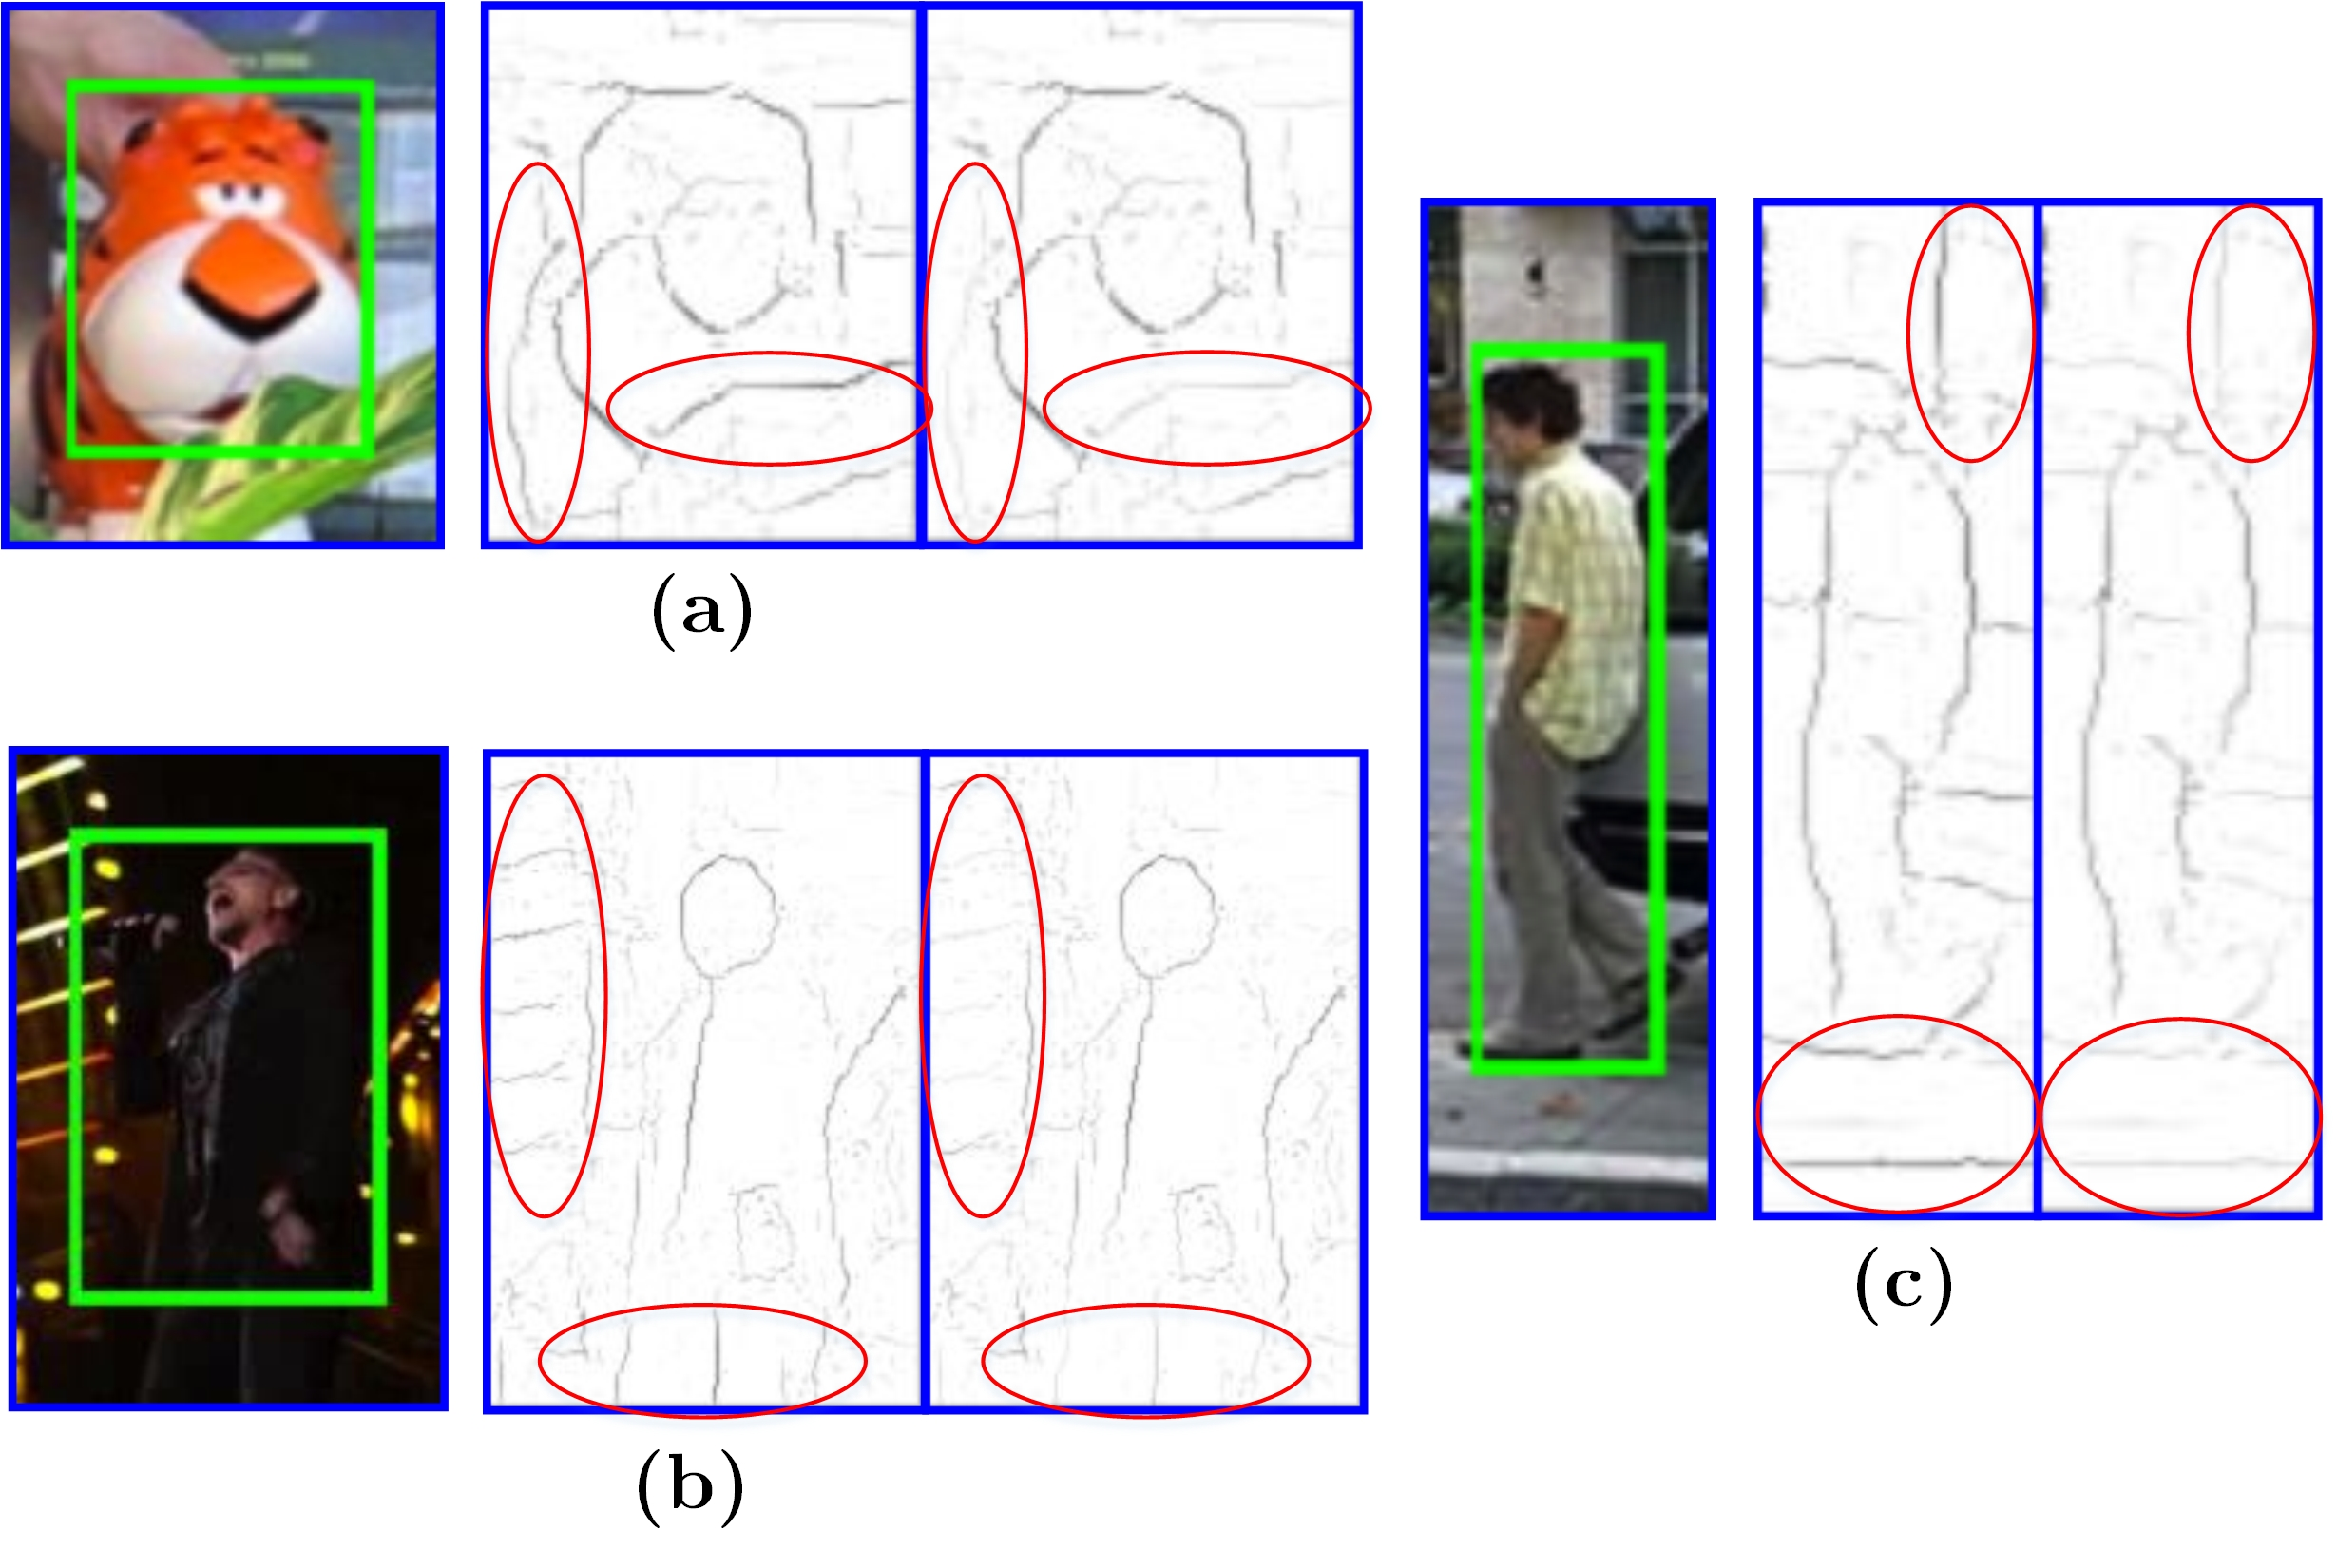
\includegraphics[width=10cm]{Fig2.jpg}
	\caption{背景抑制的可视化效果}
	\label{punish}
\end{figure}



\section{跟踪器中目标候选生成器的适配}
\label{generatoradaptsec}
本节的目的有两个方面。
一方面,本节通过将不同的目标候选生成器向跟踪任务进行适配,并利用上一章的方法嵌入跟踪器中,
将揭示目标候选质量和跟踪精度间的关系。
另一方面,通过对比嵌入不同目标候选生成器后的跟踪器精度,将证明本章对EdgeBoxes的优化是非常有效的。

在进行本节的工作前,目标候选对于跟踪器的作用是不明朗的。
如果目标候选在物体跟踪中没有作用,
那么不使用目标候选生成器,仅仅在目标初步位置附近进行随机采样,也能获得近似的跟踪精度提升。
目标候选生成器Bing\upcite{bing}就是一个典型的例子。
有文献指出,Bing的分类器并没有实际作用\upcite{crackingbing}。
如果无视图像实际内容,单纯按照一定模式采样目标候选,也可以生成同等质量的目标候选。
本节的工作和对应的实验结果将证明,目标候选对于跟踪精度的影响很大,
且目标候选的质量和跟踪器的准确性是正相关的。

在对目标候选生成器进行适配之前,本节将首先介绍目标候选的质量度量方法。
目标候选的初衷是为物体检测提供初步的候选区域,以加速对所有候选区域的分类过程。
因此,评价一个目标候选生成器提取的目标候选质量的最可靠标准就是,将其嵌入物体检测器后获得的物体检测精度(通常用召回率来度量)。
但是,由于物体检测器本身具有不同的质量和特点,适用的目标候选生成器也不尽相同,因此上述标准难以实际应用。
\cite{dpsurvey}率先提出了一种新的目标候选质量度量\pozhehao 平均召回率(Average Recall)图。
要得到平均召回率图无需真正地进行物体检测,其计算方式如下。
在物体检测测试集中,将每幅图像输入目标候选生成器。
然后将测试集的正确结果(准确包围各个物体的边界框)和所有目标候选进行对比,
如果某物体边界框和任意一个目标候选边界框的重叠率(IoU)超过一个阈值(记为$IoU\_threshold$),
则认为目标候选成功覆盖了该物体。
将被覆盖的物体数目除以所有物体数目,即得到了召回率(Recall)。
显然,生成的目标候选数量不同,或者$IoU\_threshold$不同,都将得到不同的召回率。
通过控制目标候选生成器的参数,令其生成一定数量的目标候选,
然后将$IoU\_threshold$分别设置为$0.5\sim 1$(以$0.1$为步长),计算其召回率。
对不同$IoU\_threshold$下的召回率取平均值,即可得到平均召回率。
最后,令目标候选生成器生成不同数量的目标候选,并将目标候选数量(沿横坐标)和对应的平均召回率(沿纵坐标)绘制成图表,
即得到了平均召回率图。
通过平均召回率图,将能够明确地判断出不同目标候选生成器生成的目标候选质量。

\cite{dpsurvey}通过在三大物体检测数据集(PASCAL VOC 2007、ImageNet、MS COCO)上计算平均召回率图,
将常用的目标候选生成器的质量和速度总结出来,如表\ref{methods-comparison}所示。
表\ref{methods-comparison}中列出了不同目标候选生成器所属的类别、在一帧图像上生成目标候选所需的平均时间、
以及生成的目标候选质量等级。
质量等级按照从低到高的顺序,逐级标记为``$\cdot$''、``$\star$''、``$\star\star$''和``$\star\star\star$''。

\begin{table}[htb]
\begin{centering}
\caption{常用目标候选生成器的质量和速度对比\upcite{dpsurvey}}
\label{methods-comparison}
\begin{tabular}{ccccccccccc}
\hline
{\small{}名称} &  & {\small{}类别} & {\small{}平均时间开销(秒)} & {\small{}目标候选质量}\tabularnewline
% &  &  & {\small{}(单位:秒)} & \tabularnewline
\hline 
\texttt{\small{}Bing }{\small{}\upcite{bing}} &  & {\small{}窗口评分} & 0.2 & $\cdot$\tabularnewline
\texttt{\small{}CPMC }{\small{}\upcite{cpmc}} &  & {\small{}区域分组} & 250 & $\star$\tabularnewline
\texttt{\small{}EdgeBoxes }{\small{}\upcite{edgeboxes}} &  & {\small{}窗口评分} & 0.3 & $\star\star\star$\tabularnewline
\texttt{\small{}Endres }{\small{}\upcite{endres}} &  & {\small{}区域分组} & 100 & $\star\star$\tabularnewline
\texttt{\small{}Geodesic }{\small{}\upcite{geodesic}} &  & {\small{}区域分组} &  1 & $\star\star$\tabularnewline
\texttt{\small{}MCG }{\small{}\upcite{mcg}} &  & {\small{}区域分组} & 30 & $\star\star\star$\tabularnewline
\texttt{\small{}Objectness }{\small{}\upcite{objectness}} &  & {\small{}窗口评分} & 3 & $\cdot$\tabularnewline
\texttt{\small{}Rahtu }{\small{}\upcite{rahtu}} &  & {\small{}窗口评分} &  3 & $\star$\tabularnewline
\texttt{\small{}RandomizedPrim's }{\small{}\upcite{randomizedprim}} &  & {\small{}区域分组} & 1 & $\star\star$\tabularnewline
\texttt{\small{}Rantalankila }{\small{}\upcite{rantalankila}} &  & {\small{}区域分组} & 10 & $\star\star$\tabularnewline
\texttt{\small{}Rigor }{\small{}\upcite{rigor}} &  & {\small{}区域分组} & 10 & $\star\star$\tabularnewline
\texttt{\small{}SelectiveSearch }{\small{}\upcite{selectivesearch}} &  & {\small{}区域分组} & 10 & $\star\star\star$\tabularnewline
\hline 
\texttt{\small{}Baseline\_Gaussian} &  & {\small{}基准}  &  0 & $\star$\tabularnewline
\texttt{\small{}Baseline\_Uniform} &  & {\small{}基准}  &  0 & $\cdot$\tabularnewline
\end{tabular}
\par\end{centering}
\end{table}

通过分析表\ref{methods-comparison},本节将4个目标候选生成器\pozhehao EdgeBoxes、Geodesic、Objectness和Bing,
以及两个基准方法\pozhehao 高斯随机采样(Gaussian)和均匀随机采样(Uniform),分别嵌入跟踪器中。
嵌入不同目标候选生成器的方法和上一章\ref{wholeprocesssec}节一样,
即将算法\ref{algorithm}第4步的EdgeBoxes替换为其它生成器。
跟踪器部分,包括图像特征整合、鲁棒模型更新以及目标候选过滤等,均不作任何修改。
此外,本节还将未嵌入任何目标候选生成器的跟踪器也考虑进来。
最后,再将本章加入背景抑制优化后的EdgeBoxes也嵌入跟踪器中,总共得到8个跟踪器。
参数的设置均保持与上一章\ref{param_setup}节一致。

之所以选用上述目标候选生成器,最重要的原因在于它们生成目标候选的时间开销较少。
一些常用的目标候选生成器,如SelectiveSearch、MCG和CPMC,
虽然也能够生成较高质量的目标候选,但是时间开销太大,无法满足跟踪任务对时效性的需求,因此本节不作考虑。
另一个原因在于目标候选的质量。
本节希望分析出不同候选质量对于跟踪精度的影响,因此选择的生成器覆盖了不同的目标候选质量等级。

在将各个目标候选生成器嵌入跟踪器之前,需要对它们进行适配。
这里的适配指的是对生成器的参数进行调整,或者是对可选模块进行替换,
但是不对其核心算法进行任何修改。
进行适配的目的有两个,一是通过分析参数的实际作用来适当地调优参数,以在保证足够跟踪速度的同时,
尽量提高跟踪精度;
二是通过调整对生成候选数目有直接或者间接影响的参数,让各个生成器生成的目标候选数量相近(120个左右),
以保证跟踪精度对比的公平性。
针对各个目标候选生成器的具体适配工作介绍如下:
\begin{compactitem}
\item \textbf{EdgeBoxes}
\end{compactitem}

参数的设置参见上一章\ref{param_setup}节。
嵌入了适配后的EdgeBoxes的跟踪器实际上就是上一章得到的KCFDP。
\begin{compactitem}
\item \textbf{Geodesic}
\end{compactitem}

本节将基本沿用\cite{dpsurvey}中建议的参数设置,仅做一些细微改动。
Geodesic的第一步是利用多尺度的结构化边缘提取器\upcite{structurededge}来提取边缘,并将图像分割为超像素。
考虑到多尺度结构化边缘提取器的时间开销过大,并且跟踪任务中输入Geodesic的图像块的尺度通常较小,无需多尺度边缘提取,
因此这里将其替换为单尺度的结构化边缘提取器。
在进行前背景分割时,本节仅放置20个种子点来构成前景,原因在于目标物体通常占据了输入图像块的大部分,20个种子点足够命中目标物体。
根据\ref{backsuppresssec}节开头的分析,目标物体通常被完全包含在输入图像块中,因此本节将输入图像块的边界和一个空集合作为背景。
相比完整图像,输入图像块中的物体数量要少得多,故用于合并超像素的``SDGT等级集合''的数量被设置为5个。
\begin{compactitem}
\item \textbf{Objectness}
\end{compactitem}

Objectness为了计算``物体性'',在评分函数中使用了多种线索。
由于其算法本身开销较大,本节仅采用其中最有代表性的两种线索,即多尺度显著性(Multi-Scale Saliency,MS)和
跨越的超像素数目(Superpixels Straddling,SS)。
虽然仅使用了两种线索,但是根据\cite{objectness}中的实验,此时Objectness已经可以达到与使用全部线索时相当的性能。
考虑到跟踪任务中输入的图像块要简单得多,本节将Objectness的初步采样窗口数目降低到$1200$个。配合显著性检测,
该数目足以覆盖目标物体。
基于同样原因,计算多尺度显著性线索时使用的尺度集合缩小为$\{16, 32\}$。
在最后的非极大值抑制步骤中,本节将IoU阈值从$0.5$提升到$0.7$,以提高覆盖目标物体的目标候选的准确度。
该步骤中的最大输出窗口数也更改为$120$,以确保它生成的目标候选数量和其它目标候选生成器相近。
\begin{compactitem}
\item \textbf{Bing}
\end{compactitem}

Bing主要基于一个训练出来的线性分类器,因此可供调节的参数很少。
本节保留\cite{bing}中推荐的参数设置,并采用其Matlab封装\upcite{bingImpl}后的版本。
线性分类器的模型直接采用\cite{bingImpl}中在PASCAL VOC 2007数据集上训练得到的结果。
此外,本节将非极大值抑制大小(Non-Maximal Suppression Size,NSS)减小为$1$,以产生更为密集的目标候选,
从而提高覆盖目标物体的目标候选的准确度。
\begin{compactitem}
\item \textbf{Baseline\_Uniform}
\end{compactitem}

该目标候选生成器即是表\ref{methods-comparison}中的Baseline\_Uniform。
它在\cite{dpsurvey}中作为一个测试基准,用于和其它目标候选生成器进行对比。
Baseline\_Uniform认为,图像中物体的相对中心位置、面积的平方根、宽高比的对数都是均匀分布的,
并根据PASCAL VOC 2007的正确结果统计出它们的范围。
在生成目标候选时,Baseline\_Uniform无视图像实际内容,
仅按照统计结果对相对中心位置、面积的平方根、宽高比的对数进行随机均匀采样,
并输出对应的边界框作为目标候选。
本节将采样$120$次,即生成$120$个目标候选。
\begin{compactitem}
\item \textbf{Baseline\_Gaussian}
\end{compactitem}

该目标候选生成器即是表\ref{methods-comparison}中的Baseline\_Gaussian。
类似Baseline\_Uniform,它也是\cite{dpsurvey}中的一个测试基准。
不同的是,它认为图像中物体的相对中心位置、面积的平方根、宽高比的对数是服从一个多元高斯分布(Multi-Variate Gaussian)的,
并根据PASCAL VOC 2007的正确结果估计出了该多元高斯分布的参数。
在生成目标候选时,Baseline\_Gaussian同样无视图像实际内容,
仅按照该多元高斯分布对相对中心位置、面积的平方根、宽高比的对数进行随机采样,
并输出对应的边界框作为目标候选。
同理,将采样$120$次以生成$120$个目标候选。

在经过上述的适配之后,6个目标候选生成器将被分别嵌入跟踪器中,并与嵌入了本章优化后的EdgeBoxes的跟踪器,
以及未嵌入目标候选生成器的跟踪器进行性能对比。
对比的结果和相关分析将在\ref{dpeffectsec}节中进行介绍。




\section{实验评测与分析}
\subsection{实验设置}
为了与上一章的KCFDP区分开来,这里把沿用了上一章方法,并嵌入了本章优化后的EdgeBoxes的跟踪器
命名为``KCFDPT(Kernelized Correlation Filter with Detection Proposals for Tracking)''。
KCFDPT的参数设置保持和上一章\ref{param_setup}节一样,但是为了测试这些参数的作用,
以及证明这些参数设置的有效性,本节将进行额外的参数敏感性分析(Parameter Sensitivity Analysis)。
由于EdgeBoxes采用C++进行实现,因此本章中EdgeBoxes的背景抑制优化也使用C++实现。
其余部分的实现均保持不变,直接采用上一章的程序。
硬件和软件环境也保持和上一章相同。

主要测试集仍然采用上一章的OTB以及它的两个子集,即``尺度变化''子集和``宽高比变化''子集。
此外,为了测试KCFDPT的通用性,本节还将在VOT 2014测试集上进行额外的实验。
对照组也基本和上一章相同,只是增加了较新的``类相关滤波跟踪器''STC\upcite{stc},
以及嵌入了不同目标候选生成器的跟踪器。
至于评价标准,在OTB测试集上,本节仍然沿用上一章\ref{evalcriteriasec}节的准确率图和成功率图。
此外,除了这两类统计图,本节还将进行数值化的距离精度和重叠精度对比。
在VOT 2014测试集上,由于它提供了自己的评价标准,故将在对应章节进行专门介绍。

本节的实验评测主要分为两个部分:一部分是将嵌入了不同目标候选生成器的跟踪器进行对比,
以分析目标候选在跟踪器中的作用,并同时证明本章对EdgeBoxes的背景抑制优化的有效性;
另一部分是将KCFDPT和不同的跟踪器进行对比,以体现优化后的EdgeBoxes对于跟踪任务的较高适应性。

\subsection{跟踪器中目标候选的作用分析}
\label{dpeffectsec}
\begin{figure}[htb]
  \centering
  \subfloat[针对尺度适应力的准确率图]{%
    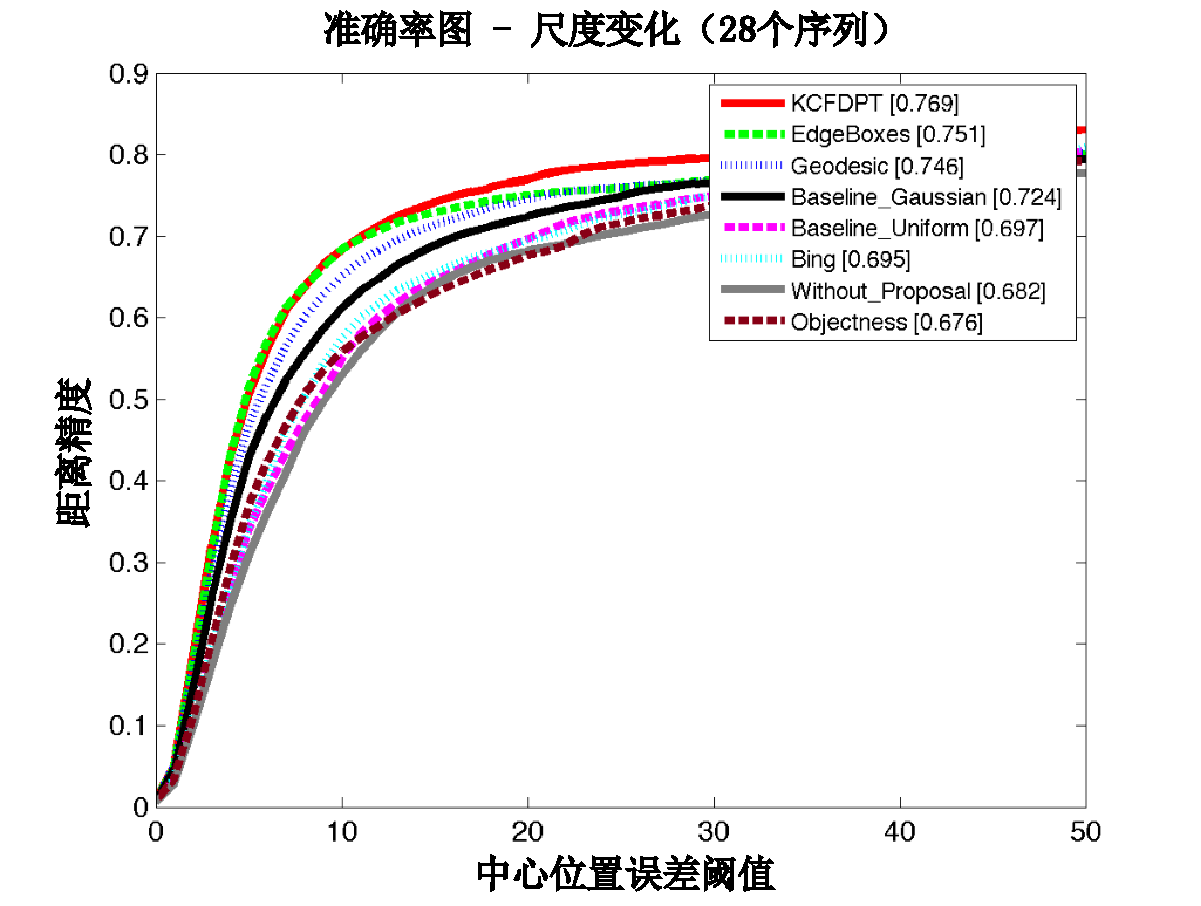
\includegraphics[height=8cm,width=10cm]{resultdpscale-1.pdf}}\hspace{-2.5cm}
  \newline
  \subfloat[针对尺度适应力的成功率图]{
    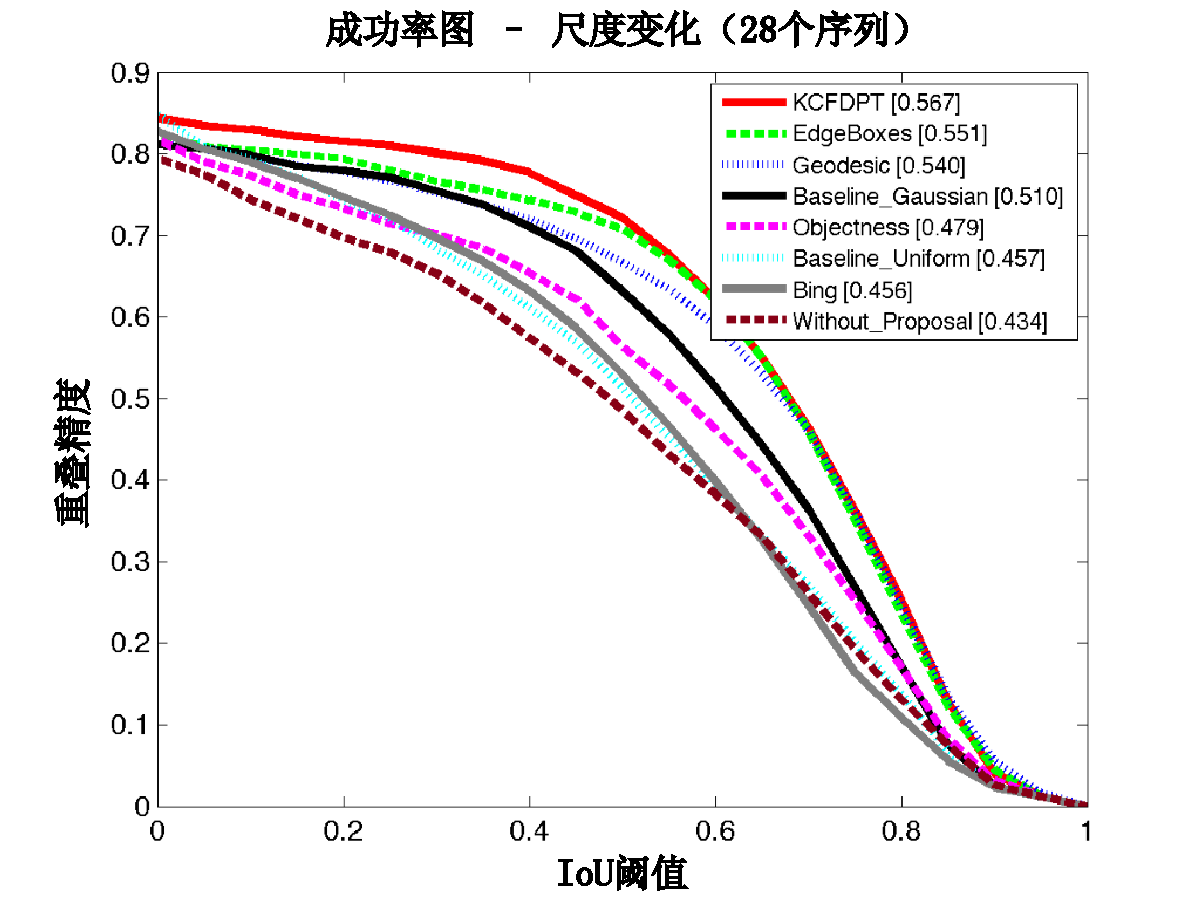
\includegraphics[height=8cm,width=10cm]{resultdpscale-2.pdf}}
  \caption{嵌入不同目标候选生成器后的尺度适应力对比}
  \label{resultdpscale}
\end{figure}

\begin{figure}[htb]
  \centering
  \subfloat[针对宽高比适应力的准确率图]{%
    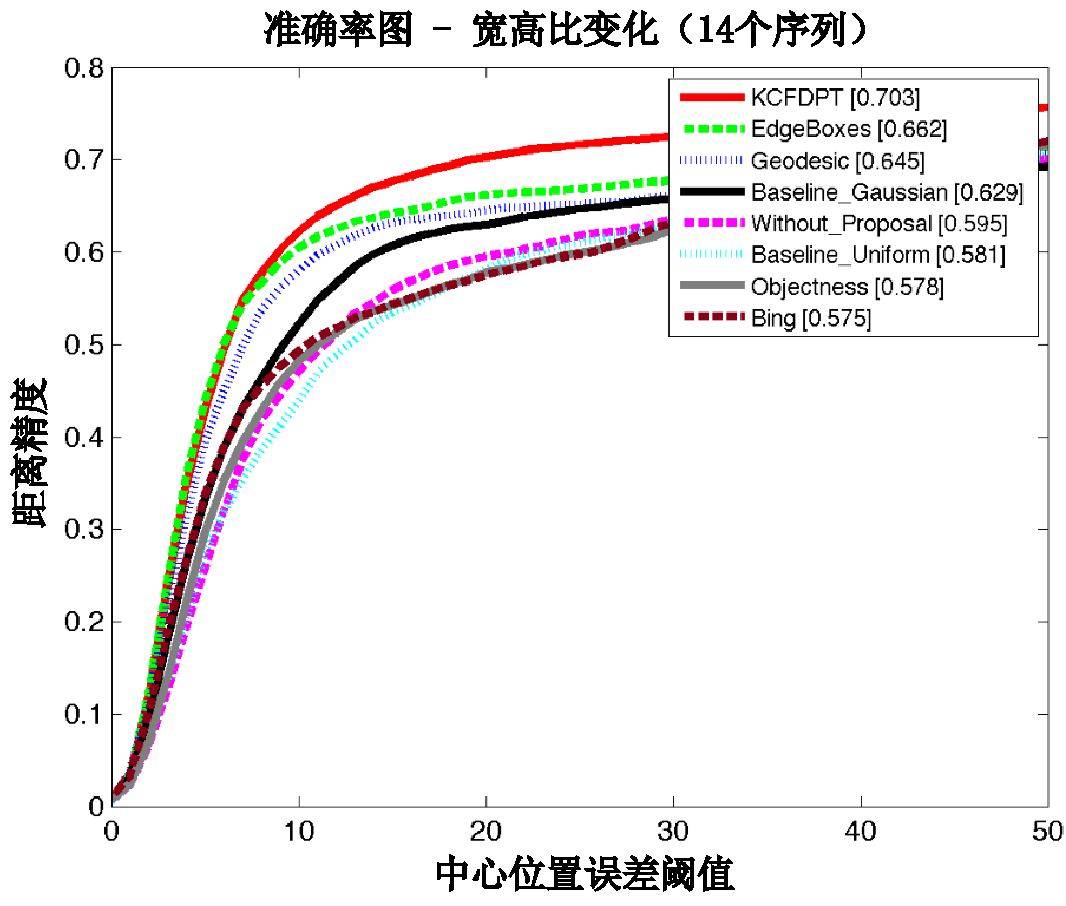
\includegraphics[width=9cm]{resultdpas-1.pdf}}\hspace{-2.5cm}
  \newline
  \subfloat[针对宽高比适应力的成功率图]{
    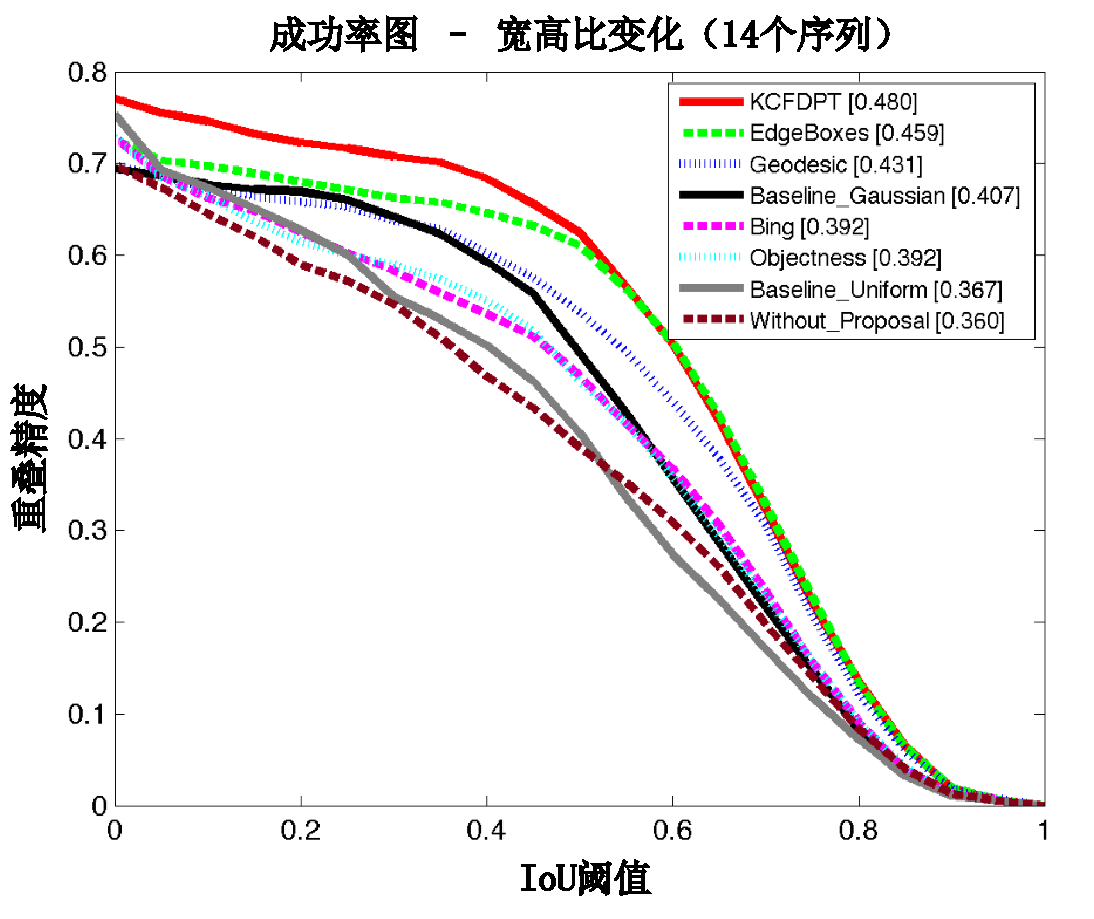
\includegraphics[width=9.3cm]{resultdpas-2.pdf}}
  \caption{嵌入不同目标候选生成器后的宽高比适应力对比}
  \label{resultdpas}
\end{figure}

\begin{figure}[htb]
  \centering
  \subfloat[完整测试集上的准确率图]{%
    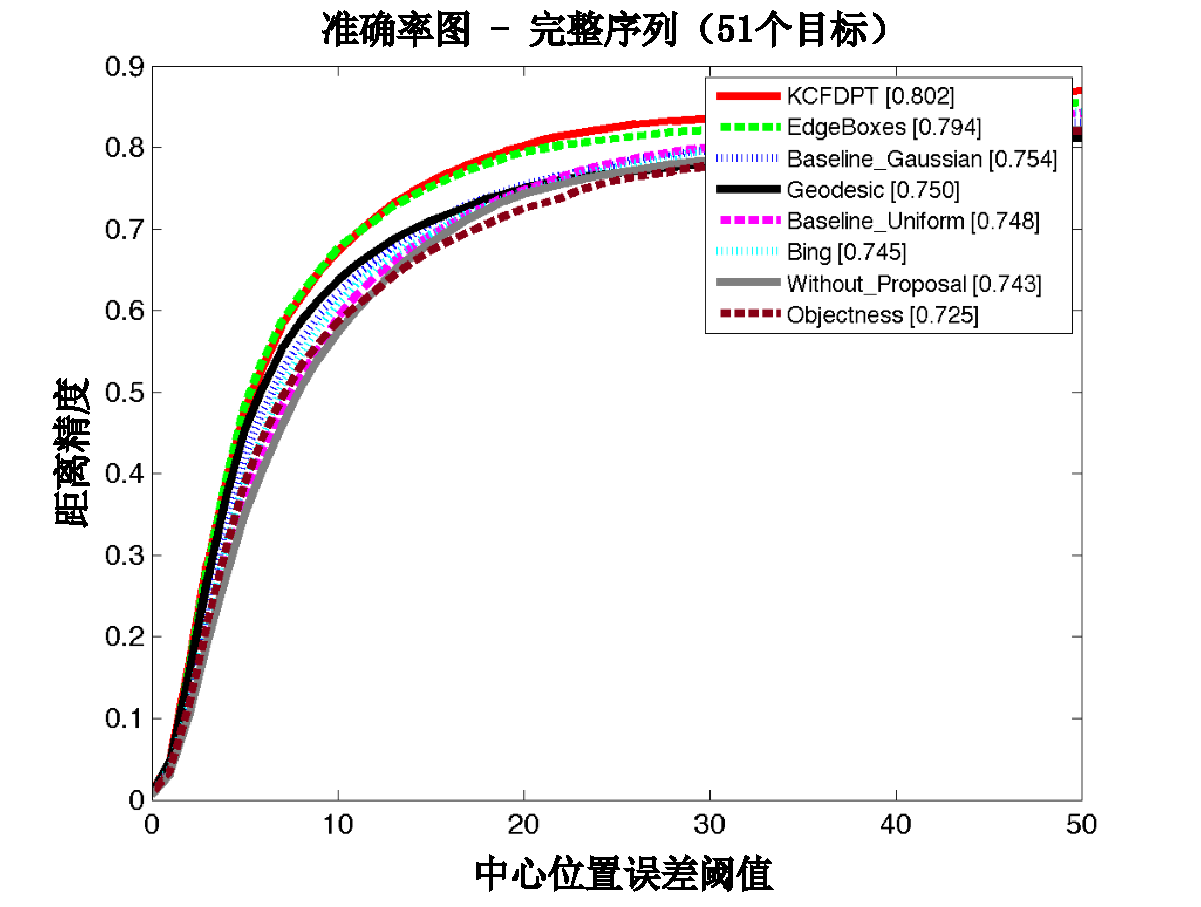
\includegraphics[height=8cm,width=10cm]{resultdpall-1.pdf}}\hspace{-2.6cm}
  \newline
  \subfloat[完整测试集上的成功率图]{
    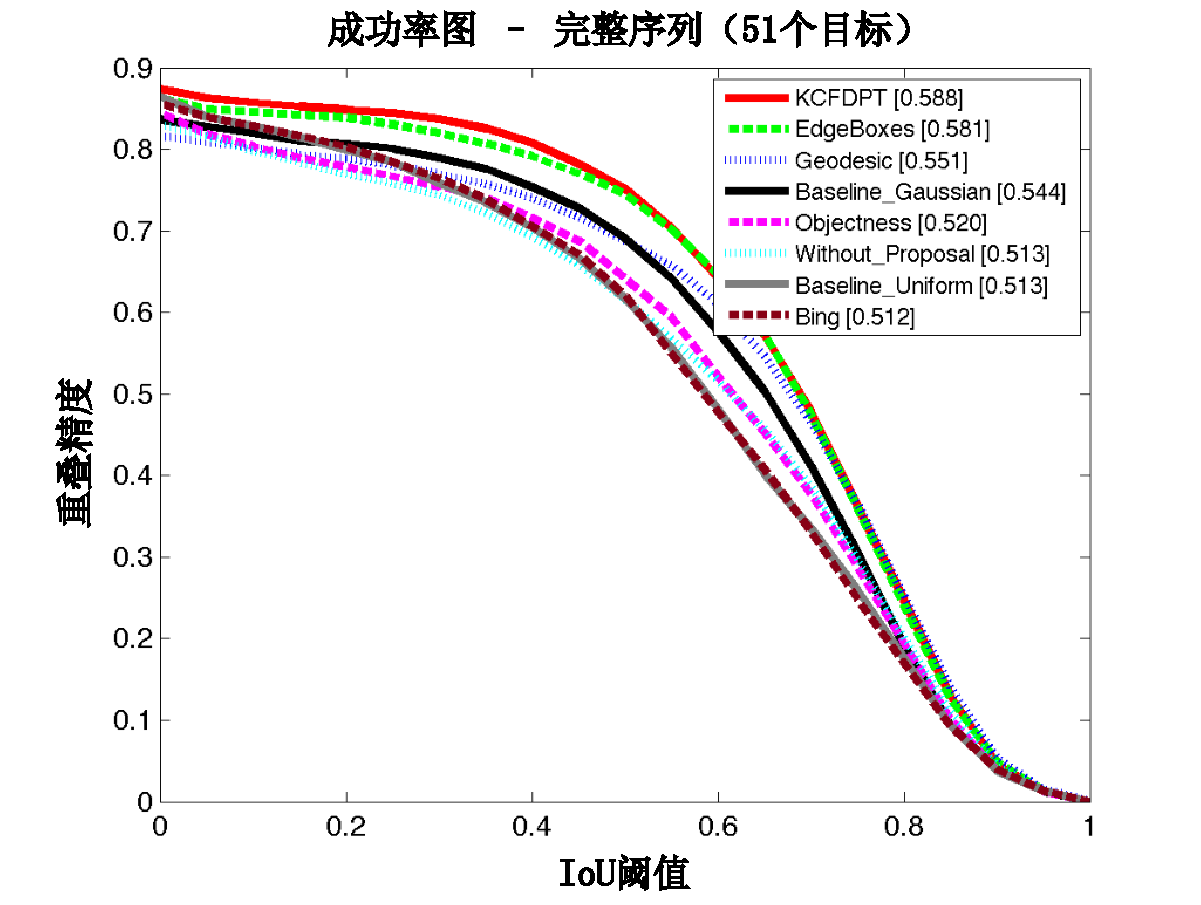
\includegraphics[height=8cm,width=10cm]{resultdpall-2.pdf}}
  \caption{嵌入不同目标候选生成器后的整体性能对比}
  \label{resultdpall}
\end{figure}

\ref{generatoradaptsec}节中,通过将6个不同的目标候选生成器面向跟踪任务进行适配,并嵌入跟踪器中,得到了6个新的跟踪器。
这里将它们用各自所包含生成器进行命名。
此外,加上未使用目标候选的跟踪器(记为Without\_Proposal)以及KCFDPT,一共有8个跟踪器。
这8个跟踪器在OTB的``尺度变化''子集、``宽高比变化''子集和完整测试集上的运行结果(准确率图和成功率图)
分别如图\ref{resultdpscale}、图\ref{resultdpas}、和图\ref{resultdpall}所示。

根据表\ref{methods-comparison}中目标候选生成器所生成的目标候选质量排名,
EdgeBoxes、Geodesic和Baseline\_Gaussian依次取得了从高到低的前三名。
而余下的3个生成器,Bing、Objectness和Baseline\_Uniform都将生成类似质量的较差的目标候选。
再观察本小节的3个实验结果图,可以清晰地看出,该目标候选质量排名和对应跟踪器的准确性排名十分吻合。
因此可以得出结论:目标候选质量与嵌入目标候选生成器后的跟踪精度间存在着正相关关系。
从实验结果图还可以看出,不同目标候选生成器所带来的跟踪精度差别十分显著,
嵌入一些质量较差的目标候选生成器甚至会产生副作用,使得跟踪精度低于Without\_Proposal。
这一现象证明,目标候选在视觉物体跟踪中有着重要的作用。
要提升跟踪精度,必须选用质量较高的目标候选生成器,并进行有针对性的优化。

相比其它7个跟踪器,KCFDPT无论在尺度和宽高比适应力上(图\ref{resultdpscale}和\ref{resultdpas}),
还是在面对各种跟踪障碍的鲁棒性上(图\ref{resultdpall}),均是最优的。
这充分证明了本章优化后的EdgeBoxes是最适于跟踪任务的。
KCFDPT和Without\_Proposal间的明显性能差距也显示了优化后的EdgeBoxes所带来的巨大性能提升。
此外,KCFDPT相对于EdgeBoxes(KCFDP)的性能提升显示了本章背景抑制优化的有效性。
但是,这一性能提升在图\ref{resultdpall}中变得不够明显,原因在于背景抑制并不能解决所有的跟踪障碍,
例如``快速运动(Fast Motion)''将导致初步目标位置的判定不够准确,
``离开视野(Out of View)''将导致目标物体无法被完全包含在目标候选生成器的输入图像块中。

为了更进一步地分析不同目标候选生成器在跟踪器中的作用,
表~\ref{dpstat}给出了各个跟踪器在整个OTB测试集上的一些统计数据。
各个目标候选生成器在一帧中平均生成的候选数量是近似的,这保证了本节性能对比的公平性。
而目标候选在过滤前后的巨大数量差别,充分证明了目标候选过滤步骤的有效性。
即使是在低功耗CPU上运行,KCFDPT的平均跟踪速度也达到了20.4 FPS,足以说明其高效性。
此外,通过对比KCFDPT和EdgeBoxes(KCFDP)的跟踪速度,可以看出背景抑制优化带来的额外时间开销几乎是可以忽略不计的。

\begin{table*}
	\centering
	\begin{tabular}{| p{1.3in} | p{0.9in}<{\centering} | p{0.9in}<{\centering} | p{0.9in}<{\centering} |}
		\hline
		Tracker with detection proposal & Avg. tracking speed (FPS) & Avg. proposal \# before rejection & Avg. proposal \# after rejection \\
		\hline
		KCFDPT & 20.4 & 103.34  & 4.43 \\
		\hline
		EdgeBoxes & 20.8  & 103.00  & 4.38 \\
		\hline
		Geodesic & 14.4 & 127.07  & 4.78 \\
		\hline
		Objectness & 6.5  & 104.95  & 1.37 \\
		\hline
		Bing & 30.9  & 133.22 & 2.32 \\
		\hline
		Baseline\_Uniform & 25.1  & 120.00  & 3.17 \\
		\hline
		Baseline\_Gaussian & 27.2  & 120.00  & 2.80 \\
		\hline
		Without\_Proposal & 112.2  & --  & -- \\
		\hline
	\end{tabular}
	\caption{Each tracker's average tracking speed and average proposal number per frame before and after proposal rejection on the whole 50-sequence dataset. Please note that the tracking speed is affected by both proposal generation speed and proposal number after rejection.}
	\label{dpstat}
\end{table*}

\subsection{跟踪器中目标候选的优化效果评测}
\subsubsection{统计图对比评测}
以下均翻译ijcv论文
\subsubsection{数值化对比评测}
\subsubsection{VOT测试集上的对比}
\subsubsection{参数敏感性分析}
\label{parameter-sensitivity}

\section{小结}